\documentclass[%
	final, %
	% draft, % Grafische Elemente durch graue Boxen ersetzen (beschleunigt Kompilieren)
	% 8pt, % Zu klein, erfordert Paket extsize
	% 9pt, % Zu klein, erfordert Paket extsize
	% 10pt, % für Folien mit sehr viel Text
	9pt, % Standardschriftgröße
	% 12pt, % etwas größer und daher besser zu lesen
	% 14pt, % deutlich größer, erfordert Paket extsize
	% 17pt, % PowerPoint Standardschriftgröße, erfordert Paket extsize
	% 20pt, % sehr groß, erfordert Paket extsize
	% trans,% Zum Erstellen von Overhead Folien
	% handout, % Erstellen eines Handouts
	% article,% Erstellen eines Artikels
 	% compress, % Die Navigation in der Kopfzeile wird komprimiert dargestellt
	t, % Place text of slides at the (vertical) top of the slides
	% c, % Place text of slides at the (vertical) center of the slides
	% color={}, % list of options for color
	xcolor={table,dvipsnames}, % Optionen für xcolor übergeben
	% hyperref={}, % list of options for hyperref
	% envcountsect, % Causes theorems, definitions, and so on to be numbered locally to each section.
	% notheorems, % Switches off the definition of default blocks like theorem
	% noamsthm, % Does not load amsthm and also not amsmath
	% ucs, % lädt ucs Paket
	% utf8, % lädt utf8x Paket von ucs (utf8 enconding)
	% dvips, % erzwingt das Laden des dvips Treibers - idR nicht nötig!
	% usepdftitle=false, % Suppresses the automatic generation of title and author entries in the pdf document information.
	% ignorenonframetext, % suppresses content created for the article mode ??
	show notes, % enables Notes
	% leqno,
	% fleqn,
]{beamer}[2007/03/11] % Minimum necessary version due to severe bugs in version 3.06 !!!

% ~~~~~~~~~~~~~~~~~~~~~~~~~~~~~~~~~~~~~~~~~~~~~~~~~~~~~~~~~~~~~~~~~~~~~~~~
% Fonts Fonts Fonts
% ~~~~~~~~~~~~~~~~~~~~~~~~~~~~~~~~~~~~~~~~~~~~~~~~~~~~~~~~~~~~~~~~~~~~~~~~
\usepackage[T1]{fontenc} % T1 Schrift Encoding
\usepackage{textcomp}	 % additional symbols (Text Companion font extension)
 
 
% \usepackage{lmodern}               %% --- Latin Modern
\usepackage{mathptmx}              %% --- Times mit Matheschriften
% \usepackage{mathpazo}              %% --- Palantino
% \usepackage{charter}               %% --- Charter
% \usepackage{bookman}               %% Bookman (lädt Avant Garde !!)
% \usepackage{newcent}               %% New Century Schoolbook (lädt Avant Garde !!)
 
% \usepackage{bera}
\usepackage[scaled=.90]{helvet}    %% --- Helvetica (Arial)
% \usepackage{cmbright}              %% --- CM-Bright (eigntlich eine Familie)
% \usepackage{tpslifonts}            %% --- (Font for Slides)
% \usepackage{avant}      	          %% --- Avantgard
%
\usepackage{courier}               %% --- Courier
%\usepackage[scaled=0.9]{luximono}  	 %% --- Luxi Mono

% *** Sprache *****************************
\usepackage[utf8]{inputenc}
\usepackage[T1]{fontenc}
\usepackage[ngerman]{babel}

\usepackage[%
   %final,
   %draft % do not include images (faster)
]{graphicx}
\usepackage{subfigure}
 
\usepackage{xcolor}
\definecolor{boxheadcol}{RGB}{59, 91, 134}
\definecolor{boxcol}{gray}{.9}

\definecolor{avedo}{RGB}{59, 91, 134}
\definecolor{darkgray}{RGB}{69,69,69}
\definecolor{lightgray}{gray}{.9}
\definecolor{darkblue}{RGB}{59, 91, 134}
\definecolor{fgcgray}{rgb}{0.4, 0.4, 0.4}
\definecolor{bgctitle}{RGB}{59, 91, 134}
\definecolor{fgctitle}{rgb}{0.99, 0.99, 0.95}
 
\usepackage{tabularx}   % Erweiterte Tabellen Optionen
\usepackage{booktabs}
\usepackage{multicol}

\usepackage{amssymb,amsmath}
\usepackage{listings}
\usepackage{hyperref}
 
\definecolor{dkgreen}{rgb}{0,0.6,0}
\definecolor{gray}{rgb}{0.5,0.5,0.5}
\definecolor{mauve}{rgb}{0.58,0,0.82}

\lstset{ %
  language=Java, % the language of the code
  basicstyle=\tiny, % the size of the fonts that are used for the code
  numbers=left, % where to put the line-numbers
  numberstyle=\tiny\color{gray}, % the style that is used for the line-numbers
  stepnumber=5, % the step between two line-numbers. If it's 1, each line
  numbersep=5pt, % how far the line-numbers are from the code
  firstnumber=1,
  numberfirstline=false,
  backgroundcolor=\color{white}, % choose the background color. You must add \usepackage{color}
  showspaces=false, % show spaces adding particular underscores
  showstringspaces=false, % underline spaces within strings
  showtabs=false, % show tabs within strings adding particular underscores
  tabsize=3, % sets default tabsize to 2 spaces
  captionpos=b, % sets the caption-position to bottom
  breaklines=true, % sets automatic line breaking
  breakatwhitespace=false, % sets if automatic breaks should only happen at whitespace
  title=\lstname, % show the filename of files included with \lstinputlisting;
  keywordstyle=\color{blue}, % keyword style
  commentstyle=\color{dkgreen}, % comment style
  stringstyle=\color{mauve}, % string literal style
  escapeinside={\%*}{*)}, % if you want to add a comment within your code
  morekeywords={*,...}, % if you want to add more keywords to the set
  xleftmargin=2em,
  xrightmargin=2em,
  aboveskip=1em,
  nolol=true
}

\def\thelstlisting{}
\makeatletter
\AtBeginDocument{%
  \renewcommand \thelstlisting
       {}%
}
\makeatother

% *****************************************
% >>> Themes <<<<<<<<<<<<<<<<<<<<<<<<<<<<<<
% *****************************************
 
% \usetheme[<options>]{<name list>} 		Installs the presentation theme named <name>.
% \usecolortheme[<options>]{<name list>} Same as \usetheme, only for color themes.
% \usefonttheme[<options>]{<name>} 		Same as \usetheme, only for font themes.
% \useinnertheme[<options>]{<name>}		Same as \usetheme, only for inner themes.
% \useoutertheme[<options>]{<name>}		Same as \usetheme, only for outer themes.

 \usetheme[%
 	secheader % section im Header
]{Boadilla}

\useinnertheme{rectangles} 

\usecolortheme[%
 	named=avedo,
]{structure}

\setbeamercolor*{titlelike}{fg=white,bg=avedo}
\setbeamercolor*{title in head/foot}{fg=white,bg=avedo}
\setbeamercolor*{date in head/foot}{fg=white,bg=avedo}
\setbeamercolor*{author in head/foot}{fg=white,bg=avedo}
\setbeamercolor*{normal text}{fg=darkgray}

\setbeamercovered{transparent}




% *****************************************
% >>>> Veraendern der Schrifteinstellung definierter Elemente
% *****************************************
 
% Beispiele
% \setbeamerfont{frametitle}{size=\large}
% \setbeamerfont{frametitle}{series=\bfseries}
 
% weitere Befehle
% size= size command sets the size attribute of the beamerfont.
% size*={ size in pt }{ baselineskip }
% shape= (\itshape, \slshape, \scshape, or \upshape)
% series= (command like \bfseries.)
% family= (command like \rmfamily or \sffamily).
% family*={ family name } (For example, the family name for Times happens to be ptm. )
% parent={ parent list } specifies a list of parent fonts.
%
% Example for parent
% \setbeamerfont{parent A}{size=\large}
% \setbeamerfont{parent B}{series=\bfseries}
% \setbeamerfont{child}{parent={parent A, parent B},size=\small}
%
% \usebeamerfont{child}
% This text is small and bold.




% *****************************************
% >>>> 15.3.2    Using Beamer’s Templates
% *****************************************

\makeatletter
\AtBeginPart{%
  \addtocontents{toc}{\protect\beamer@partintoc{\the\c@part}{\beamer@partnameshort}{\the\c@page}}%
}
%% number, shortname, page.
\providecommand\beamer@partintoc[3]{%
  \ifnum\c@tocdepth=-1\relax
    % requesting onlyparts.
    \makebox[6em]{#1.} #2
    \par
  \fi
}
\define@key{beamertoc}{onlyparts}[]{%
  \c@tocdepth=-1\relax
}
\makeatother%


\makeatletter
\setbeamercolor{secsubsec}{fg=white,bg=avedo}
\setbeamertemplate{headline}
{
  \leavevmode%
  \hbox{%
  \begin{beamercolorbox}[wd=\paperwidth,ht=2.5ex,dp=1ex]{secsubsec}%
    \raggedright
    \hspace*{2em}%
    {\sffamily\scriptsize\insertpart\hfill\insertsection}%
    \hspace*{2em}%
  \end{beamercolorbox}%
  }%
}
\makeatother

\makeatletter
\setbeamercolor{frametitle}{fg=avedo,bg=white}
\setbeamertemplate{frametitle}
{\leavevmode
  \hbox{%
  \begin{beamercolorbox}[wd=\paperwidth,ht=3.5ex,dp=0.7ex]{frametitle}%
    \raggedright\hspace*{1.5em}\Large\insertframetitle
  \end{beamercolorbox}
  }%
}
\makeatother

\makeatletter
\setbeamertemplate{footline}
{
  \leavevmode%
  \hbox{%
  \begin{beamercolorbox}[wd=.333333\paperwidth,ht=2.25ex,dp=1ex,center]{author in head/foot}%
    \usebeamerfont{author in head/foot}\insertshortauthor~~\beamer@ifempty{\insertshortinstitute}{}{(\insertshortinstitute)}
  \end{beamercolorbox}%
  \begin{beamercolorbox}[wd=.333333\paperwidth,ht=2.25ex,dp=1ex,center]{title in head/foot}%
    \usebeamerfont{title in head/foot}\insertshorttitle
  \end{beamercolorbox}%
  \begin{beamercolorbox}[wd=.333333\paperwidth,ht=2.25ex,dp=1ex,right]{date in head/foot}%
    \usebeamerfont{date in head/foot}\insertshortdate{}\hspace*{4em}
  \end{beamercolorbox}}%
  \vskip0pt%
}
\makeatother

\makeatletter
\setbeamertemplate{part page}
{
  \begin{centering}
    \vskip3em\par
    \begin{beamercolorbox}[sep=16pt,center]{part title}
      \usebeamerfont{part title}\insertpart\par
    \end{beamercolorbox}
  \end{centering}
}
\makeatother

\renewenvironment{block}[1]{%
  \begin{actionenv}%
      \def\insertblocktitle{#1}%
      \par%
      \mode<presentation>{%
        \setbeamercolor{block title}{fg=white,bg=avedo}
       \setbeamercolor{block body}{fg=darkgray,bg=lightgray}
       \setbeamercolor{itemize item}{fg=avedo}
       \setbeamertemplate{itemize item}[triangle]
       \setbeamercolor{enumerate item}{fg=avedo}
       \setbeamertemplate{enumerate item}[square]
     }%
      \usebeamertemplate{block begin}}
    {\par\usebeamertemplate{block end}\end{actionenv}}

\renewenvironment{exampleblock}[1]{%
  \begin{actionenv}%
      \def\insertblocktitle{#1}%
      \par%
      \mode<presentation>{%
        \setbeamercolor{block title}{fg=white,bg=avedo}
       \setbeamercolor{block body}{fg=darkgray,bg=lightgray}
       \setbeamercolor{itemize item}{fg=avedo}
       \setbeamertemplate{itemize item}[triangle]
       \setbeamercolor{enumerate item}{fg=avedo}
       \setbeamertemplate{enumerate item}[square]
     }%
      \usebeamertemplate{block begin}}
    {\par\usebeamertemplate{block end}\end{actionenv}}

\renewenvironment{alertblock}[1]{%
  \begin{actionenv}%
      \def\insertblocktitle{#1}%
      \par%
      \mode<presentation>{%
        \setbeamercolor{block title}{fg=white,bg=avedo}
       \setbeamercolor{block body}{fg=darkgray,bg=lightgray}
       \setbeamercolor{itemize item}{fg=avedo}
       \setbeamertemplate{itemize item}[triangle]
       \setbeamercolor{enumerate item}{fg=avedo}
       \setbeamertemplate{enumerate item}[square]
     }%
      \usebeamertemplate{block begin}}
    {\par\usebeamertemplate{block end}\end{actionenv}}

\newenvironment{attrDesc}[1]{%
   \vspace{0.3cm}
   \small
   \begin{center}
      \setlength\arrayrulewidth{0.75pt}
      \arrayrulecolor{white}
      \renewcommand{\arraystretch}{1.3}
      \rowcolors{1}{boxcol}{boxcol}
      \begin{tabular}{#1}
         \rowcolor{boxheadcol}
         \rowstyle{\color{white}\bfseries\sffamily}
}{   
      \end{tabular}
   \end{center}
   \vspace{0.3cm}
}

\newcolumntype{+}{>{\global\let\currentrowstyle\relax}}
\newcolumntype{^}{>{\currentrowstyle}}
\newcommand{\rowstyle}[1]{\gdef\currentrowstyle{#1}%
#1\ignorespaces
}

\setbeamertemplate{mini frames}[box] % shows small rectangles as mini frames.
\setbeamertemplate{navigation symbols}{} % suppresses all navigation symbols:
\setbeamersize{text margin left=2em,text margin right=2em}
\setbeamertemplate{sections/subsections in toc}[square] 
\setbeamertemplate{bibliography item}[default]
\setbeamertemplate{itemize items}[triangle]
\setbeamertemplate{enumerate items}[square]

%% Eigene Definitionen ============================
%

\newcommand{\therfore}{\ding{225}\mbox{ }}
\newcommand{\verythinarrow}{\ding{221}\mbox{ }}
\newcommand{\thinarrow}{\ding{222}\mbox{ }}
\newcommand{\newarrow}{\ding{222}\mbox{ }}
\newcommand{\addspace}{\vspace{0.5\baselineskip}}



\begin{document}
 	\title{Android -- Eine Einführung}
\subtitle{Toasts \& Notifications}
\author[A. Wilhelm]{Andreas Wilhelm}
\institute[www.avedo.net]{}
\titlegraphic{}
%\date{\today}
\date{CSC Computer-Schulung \& Consulting GmbH}

\begin{frame}[plain]
  \titlepage
\end{frame}

\section[Contents]{}
\begin{frame}
	\frametitle{Contents}
	\tableofcontents[onlyparts]
\end{frame}

\part{Toasts}
\frame{\partpage}
\begin{frame}
	\frametitle{Contents}
	\tableofcontents[]
\end{frame}

\section{Überblick}
\begin{frame}
   \frametitle{Überblick}
   \begin{itemize}
      \item Nachrichten bezüglich gestarteten, laufenden oder beendeten 
         Operationen
      \item Kleine Anzeige, die nur benötigten Platz einnimmt
      \item Darunterliegende Oberfläche weiterhin nutzbar
      \item Keine Interaktion mit Toasts
   \end{itemize}

   \lstinputlisting[
      caption=Ein erster Toast,
      label={lst:FirstToast.java}]{src/java/FirstToast.java}
\end{frame}

\section{Anpassung des Layouts}
\begin{frame}
   \frametitle{Positionierung}
   \begin{itemize}
      \item Normalerweise Anzeige zentriert am unteren Bildschirmrand
      \item Änderung der Position mit \emph{setGravity()}
      \item Erstes Argument Positionierung auf Bildschirm
      \item Zweites und drittes Verschiebung
   \end{itemize}

   \lstinputlisting[
      caption=Ein zentierter Toast,
      label={lst:GravityToast.java}]{src/java/GravityToast.java}
\end{frame}

\begin{frame}
   \frametitle{Eigene Layouts}
   \begin{itemize}
      \item Eigene Layouts mit \emph{setView()} zuweisen
      \item Dabei sollte Hintergund mit Shapes deklariert werden
   \end{itemize}

   \lstinputlisting[
      language=xml,caption=Das Toast Layout,
      label={lst:toast_layout.xml}]{src/xml/toast_layout.xml}
\end{frame}

\begin{frame}
   \frametitle{Shapes}
   \lstinputlisting[
      language=xml,caption=Der Toast Hintergrund,
      label={lst:toast_shape.xml}]{src/xml/toast_shape.xml}
\end{frame}

\begin{frame}
   \frametitle{Nutzung eigenes Layouts}
   \begin{itemize}
      \item Laden des Layouts mit LayoutInflater
      \item Instanzierung eines Toasts mit Konstruktor (nicht \emph{makeText})
      \item Zuweisung des Layouts mit \emph{setView()}
   \end{itemize}

   \lstinputlisting[
      caption=Ein angepasster Toast,
      label={lst:CustomToast.java}]{src/java/CustomToast.java}
\end{frame}

\begin{frame}
   \frametitle{Screenshot}
   \begin{figure}[h!]
     \centering
     \includegraphics[width=0.7\textwidth]{pictures/custom_toast.ps}
     \caption{
        Ein eigener Toast
     }
     \label{fig:custom_toast}
   \end{figure}
\end{frame}

\begin{frame}
   \frametitle{Anmerkung}
   \begin{alertblock}{Toast Konstruktor}
		Es ist unbedingt darauf zu achten, dass der öffentliche Konstruktor der Klasse 
		Toast nur dann verwendet wird, wenn ein eigenes Layout dem Toast zugewiesen werden 
		soll. In allen anderen Fällen sollte die statische Methode \emph{makeText()} 
		verwendet werden.
   \end{alertblock}
\end{frame}

\part{Notifications}
\frame{\partpage}
\begin{frame}
	\frametitle{Contents}
	\tableofcontents[]
\end{frame}

\section{Überblick}
\begin{frame}
   \frametitle{Allgemeines}
   \begin{itemize}
      \item Nachrichten in einer von der Applikation unabhängigen Umgebung
      \item Anzeige in Bar am oberen Bildschirmrand (NotificationBar) 
      \item Zuerst nur Anzeige eines Icons
      \item Anzeige weiterer Informationen in Notification-DropDown
      \item Erstellen von Notifications mit \emph{Notification.Builder}
      \item Bestandteil der API seit Android Version 3.0
      \item Verfügbar über Android Support Library
      \item Einführung weiterer Ansichten in Android 4.1
   \end{itemize}

   \begin{alertblock}{NotificationCompat.Builder}
      \emph{Notification.Builder} wurde erst in Android 3.0 (API-Version 11) eingeführt. 
      Verwendung nur mit minimal unterstützter API-Version der Applikation 11 oder höher. 
      Unterstützung älterer API-Versionen mit NotificationCompat.Builder, der Teil 
      der Android Support Library ist.
   \end{alertblock}
\end{frame}

\begin{frame}
   \frametitle{Android Support Library}
   \begin{alertblock}{Android Support Library}
		Die Android Support Library enthält Bibliotheken, die in älteren API-Versionen 
		noch nicht zur Verfügung standen oder Werzeuge bereitstellen, die nicht Teil 
		der Standard-API sind.

		\vspace{5mm}

		Man muss allerdings bei der Entwicklung darauf achten, dass die Support Library 
		mehrere Bibliotheken mit unterschiedlichen Anforderungen an die minimal unterstützte API 
		enthält. Welche Bibliothek welche Anforderungen stellt, kann man ganz einfach der 
		Verzeichnisstruktur der Support Library entnehmen. Alle Bibliotheken mit einer 
		minimalen API-Version 4 findet man unter \emph{v4}.
   \end{alertblock}
\end{frame}

\begin{frame}
   \frametitle{Normale Notifications}
   \begin{itemize}
      \item Höhe normaler Notifications bis zu 64 dp
      \item Titel am oberen Rand
      \item Großes Icon am linken Rand
      \item Zusatztext am unteren Rand
      \item Kleine Zusatzinformation und ein kleines Icon am rechten unteren Rand
      \item Zeitpunkt am rechten oberen Rand
   \end{itemize}
\end{frame}

\begin{frame}
   \frametitle{Erweiterte Notifications}
   \begin{itemize}
      \item Eingeführt in Android 4.1
      \item Gleiches Aussehen, wie normale Notifications
      \item Können allerdings ausgeklappt werden
      \item Zustätzlicher Bereich zwischen Titelzeile und der Textzeile am unteren Rand
      \item Verschiedene Anzeigen für 
         \begin{itemize}
            \item Großes Bild
            \item Längeren Text
            \item Zeilenweiser Text (Liste)
         \end{itemize}
   \end{itemize}
\end{frame}

\section{Erstellen von Notifications}
\begin{frame}
   \frametitle{Allgemeines}
   \begin{itemize}
      \item Deklarierung mit \emph{Notification.Builder} 
      \item Erzeugen mit Methode \emph{build()}
      \item Weitergabe an System mit \emph{NotificationManager}
      \item Verschiedene Einstellung im \emph{Notification.Builder} möglich
   \end{itemize}

   \begin{attrDesc}{+p{4cm}|^p{6cm}}
      Methode & Beschreibung\\
      \hline
      \emph{setSmallIcon()} & Ein kleines Icon, dass in der NotificationBar angezeigt wird\\
      \emph{setContentTitle()} & Der Titel der Notification\\
      \emph{setContentText()} & Ein kurzer Text mit Zusatzinformationen\\
   \end{attrDesc}
\end{frame}

\begin{frame}
   \frametitle{Näheres zu Attributen}
   \begin{itemize}
      \item Zuweisung von Icons oder Sounds
      \item Zuweisung einer Aktion immer sinnvoll
      \item Aktion wird als PendingIntent an \emph{setContentIntent()} übergeben
      \item PendingIntent erlaubt anderer Applikation eine Activity zu starten
   \end{itemize}

   \lstinputlisting[
      caption=Erstellen einer Notification,
      label={lst:notificationBuilder.java}]{src/java/notificationBuilder.java}
\end{frame}

\begin{frame}
   \frametitle{Hinweise}

   \begin{alertblock}{Methode \emph{build()}}
      Seit API-Version 16 ist die Methode \emph{getNotification()} der Klasse 
      Notification.Builder als \emph{deprecated} gekennzeichnet. Man sollte 
      daher wenn möglich auf die Methode \emph{build()} zurückgreifen, die 
      allerdings in älteren Versionen nicht unterstützt wird.
   \end{alertblock}

   \begin{alertblock}{NotificationCompat.Builder}
      Seit API-Level 11 (Android Version 3.0) bietet Android die Klasse 
      \emph{TaskStackBuilder}, die sich um die Verwaltung des Backstacks 
      bei der Navaigation kümmert. Die Navigation mit Hilfe des \emph{Zurück}-Buttons 
      ist nur innerhalb einer Applikation festgelegt, aber nicht der Wechsel zwischen 
      Applikationen.

      \vspace{3mm}

      Der \emph{TaskStackBuilder} ist auch kompatibel 
      zu älteren Versionen von Android. So wird seit Android 3.0 beim Aufruf von 
      \emph{startActivities()} oder \emph{getPendingIntent(int, int)} ein 
      seperater Back-Stack angelegt, während in älteren Versionen nur die oberste 
      Activity des übergebenen Stacks ausgeführt und so die Navigation zur aufrufenden 
      Applikation ermöglicht wird.
   \end{alertblock}
\end{frame}

\begin{frame}
   \frametitle{Einbinden des \emph{TaskStackBuilders}}

   \lstinputlisting[
      caption=Einbinden des TaskStackBuilders,
      label={lst:taskStackNotification.java}]{src/java/taskStackNotification.java}
\end{frame}

\begin{frame}
   \frametitle{Screenshot}
   \begin{figure}[h!]
     \centering
     \subfigure[Icon in NotificationBar]{
       \includegraphics[width=0.49\textwidth]{pictures/notificationBar.ps}
     }\hfill
     \subfigure[Eintrag in Notification-DropDown]{
       \includegraphics[width=0.49\textwidth]{pictures/notificationDropDown.ps}
     }
     \caption{
        Notifications im Einsatz
     }
     \label{fig:notifications}
   \end{figure}
\end{frame}

\section{Verwalten von Notifications}
\begin{frame}
   \frametitle{Allgemeines}
   \begin{itemize}
      \item Benachrichtigung des Anwenders in kurzen Zeitabständen
      \item Aktualisierung von Notifications entlastet System und Anwender
      \item Bei Übergabe an das System mit \emph{NotificationManager} ID angeben
      \item System aktualisiert automatisch Notifications mit selber ID
   \end{itemize}

   \lstinputlisting[
      caption=Notifications ändern,
      label={lst:updateNotification.java}]{src/java/updateNotification.java}
\end{frame}

\begin{frame}
   \frametitle{Screenshot}
   \begin{figure}[h!]
     \centering
     \includegraphics[width=0.7\textwidth]{pictures/updateNotification.ps}
     \caption{
        Aktualisieren einer Notification
     }
     \label{fig:updateNotification}
   \end{figure}
\end{frame}

\begin{frame}
   \frametitle{Entfernen von Notifications}
   \begin{itemize}
      \item Notifications werden nur durch Benutzeraktion gelöscht
      \item Alternativ kann Notification beim anklicken gelöscht werden 
         (\emph{setAutoCancel()})
      \item Löschen durch NotificationManager mit \emph{cancelAll()} oder 
         \emph{cancel(ID)} 
   \end{itemize}
\end{frame}

\section{Prozesse und Notifications}
\begin{frame}
   \frametitle{Allgemeines}
   \begin{itemize}
      \item Anzeige einer ProgressBar in Notification
      \item Verwendung der View-Klasse ProgressBar
      \item Unterscheidung in deterministische und nicht deterministische ProgressBar
      \item Bis Android 4.0 Einbindung über eigenes Layout
      \item Seit Android 4.0 Einbindung mit \emph{setProgress()}
      \item Methode \emph{setProgress()} aktualisiert auch den Zustand
   \end{itemize}
\end{frame}

\begin{frame}
   \frametitle{Implementierung}
   \lstinputlisting[
      caption=Deterministische ProgressBar in Notifications,
      label={lst:determinateProgress.java}]{src/java/determinateProgress.java}
\end{frame}

\begin{frame}
   \frametitle{Screenshot}
   \begin{figure}[h!]
     \centering
     \subfigure[ProgressBar während des Downloads]{
        \includegraphics[width=0.49\textwidth]{pictures/determinateProgress.ps}
     }\hfill
     \subfigure[ProgressBar nach dem Download]{
        \includegraphics[width=0.49\textwidth]{pictures/determinateProgressFinished.ps}
     }
     \caption{
        Eine determistische ProgressBar
     }
     \label{fig:determinateProgress}
   \end{figure}
\end{frame}

\begin{frame}
   \frametitle{Nicht deterministische ProgressBar}
   \begin{itemize}
      \item Dritter Parameter von \emph{setProgress} ist \emph{true}
      \item Erster und zweiter Parameter werden ignoriert
   \end{itemize}

   \lstinputlisting[
      caption=Nicht deterministische ProgressBar in Notifications,
      label={lst:indeterminateProgress.java}]{src/java/indeterminateProgress.java}
\end{frame}

\begin{frame}
   \frametitle{Screenshot II}
   \begin{figure}[h!]
     \centering
     \includegraphics[width=0.7\textwidth]{pictures/indeterminateProgress.ps}
     \caption{
        Eine nicht determistische ProgressBar
     }
     \label{fig:indeterminateProgress}
   \end{figure}
\end{frame}

\begin{frame}
   \frametitle{Hinweis}
   \begin{alertblock}{Eigene Layouts}
      In älteren Android Versionen musste eine ProgressBar über ein eigenes Layout eingefügt werden. 
      Natürlich ist es auch in neueren Versionen von Android möglich eigene Layouts zu deklarieren. 
      Dabei ist allerdings darauf zu achten, dass die normale Ansicht 
      nur 64dp und die erweiterte Ansicht 256dp hoch ist.

      \vspace{5mm}

      Deklaration eines eigenen Layouts erfolgt in XML. Das Layout wird als RemoteView 
      geladen und mit \emph{setContent()} der Klasse \emph{Notification.Builder} bzw. 
      \emph{NotificationCompat.Builder} zugewiesen. Dabei sollten 
      Hintergundbilder vermieden werden, da sonst die Schrift unlesbar werden könnte. 
      Außerdem sollte auf komplexe Layouts verzichtet werden. Der Einsatz von 
      System-Ressourcen ist sehr zu empfehlen.
   \end{alertblock}
\end{frame}

\end{document}
